\section{Analysis}

\subsection{Use Case analysis}

\subsubsection{Class Candidates}

\subsubsection{Description of Classes}

\subsubsection{UML Analysis Diagram}

\subsection{Use Case Realisation}

\subsubsection{Sequence Diagrams}
A sequence diagram shows the system events for a given scenario of a use case,
and how the actor interacts with the system to solve the use case. There are two
kinds of sequence diagrams, system and operation. The system sequence diagram
displays the system as a 'black box', where the internal system events are not
shown, but only the external. This means that the diagram displays how actors
generate system events and what the system output is. Furthermore, the diagram
functions as a timeline for the system events. \\

\myworries{maybe add a system sequence diagram and explain why we used it}

The operation sequence diagram displays the system as a 'white box', where both
the internal and external system events are described, as seen in figure
\ref{figure:sequence_diagram}.

\begin{figure}[ht]
\centering 
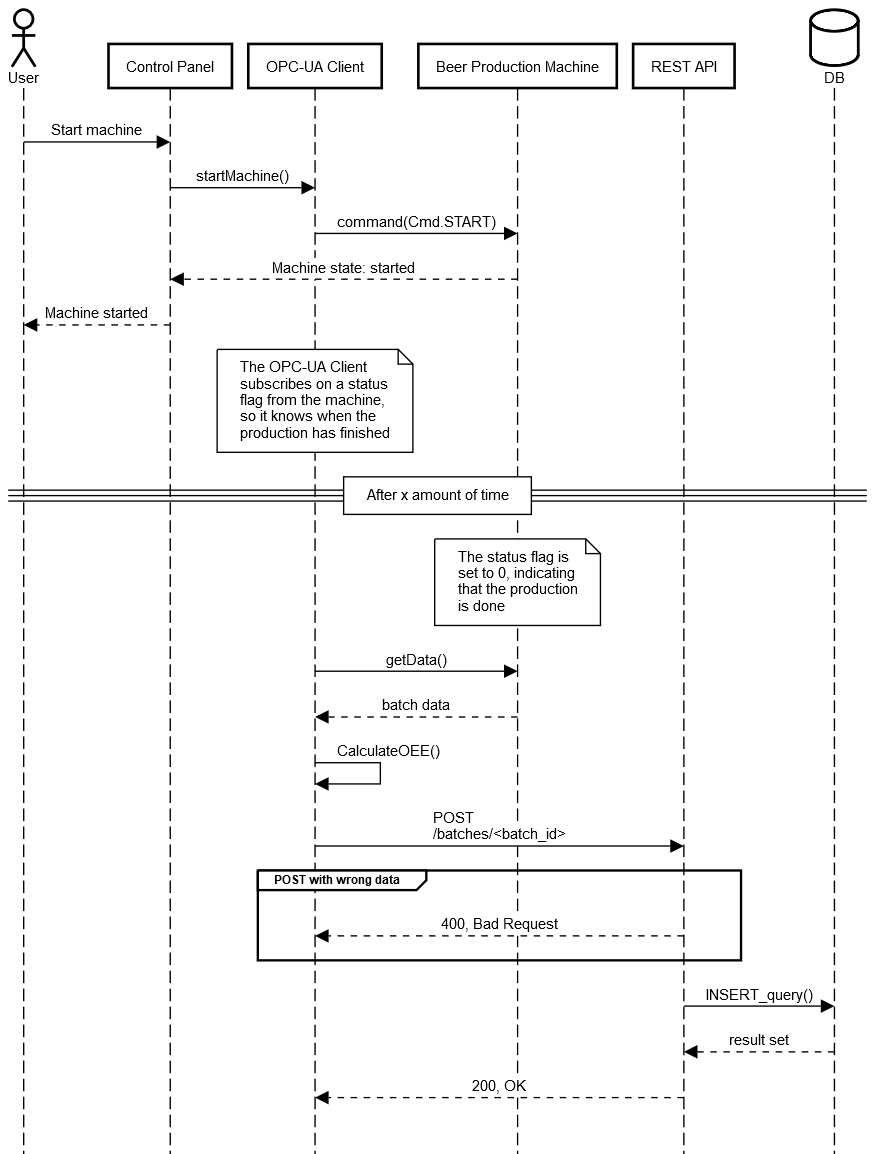
\includegraphics[scale=0.3]{images/sequence_operation/start.png}
\label{figure:sequence_diagram}
\caption{Sequence diagram: start} 
\end{figure}

This sequence diagram is used to identify system functions, as the events shown
in the diagram are the functions needed to complete the use case. In this
specific use case, the actor, the user, wants to start the beer production
machine. The user interacts with the control panel by pressing the start button,
which then sends a command to the OPC-UA client. The OPC-UA client interprets
the command as a start machine command, which triggers an event in the OPC-UA
client to send a command to the beer production machine. The beer production
machine interprets the command as a start command, which then turns on the 
machine. As a response to the user, to beer production machine sets a flag
which the control panel reacts to, and sends a message to the user. \\

When the beer production has finished, the OPC-UA client collects all relevant
data from the beer production machine. This data is used to calculate the
optimal production speed, estimate the error function, and calculate the OEE.
These calculation are used to optimise the beer production. The calculated data
and the data collected from the machine is then stored in a database. This
happens through a REST API which acts as a translater between the different 
subsystems within the MES.

\subsubsection{Operation Contracts}

\subsubsection{Updated UML Class Diagram}
